\chapter{Novel materials discovery and the new paradigm of science}
% The new paradigm of novel materials discovery
% The new paradigm of computational material science
%
% Novel discovery of
% Modern novel materials discovery

The discovery of novel materials enables the development of technological advances that are necessary to overcome challenges faced in the society, and is a principal ingredient in defining who we are and what we have become. We have witnessed the material epochs starting from the bronze age, iron age and up to the era of modern silicon technologies \cite{Jain2016, Magee2012}.

However, modern times have radically changed the methods of discovering novel materials. In the last decades, we have observed the generation of huge amounts of theoretical and experimental data, commonly known as \textit{Big data}. In the fields of computational material science, this is mainly enabled due to the success of \textit{the density functional theory} (DFT). Conversely, to keep up with the pace of data generation, a new field named \textit{Data science} combines the interdisciplinary fields of mathematics, statistics, computer science and programming to solve the challenge of extracting knowledge from unfeasibly big and complex data \cite{Agrawal2016, Schleder2019}. This is considered the fourth paradigm of science, and is visualized together with the previous paradigms of science in figure \autoref{fig:4th-paradigm}.

\begin{figure}[ht!]
  \centering
  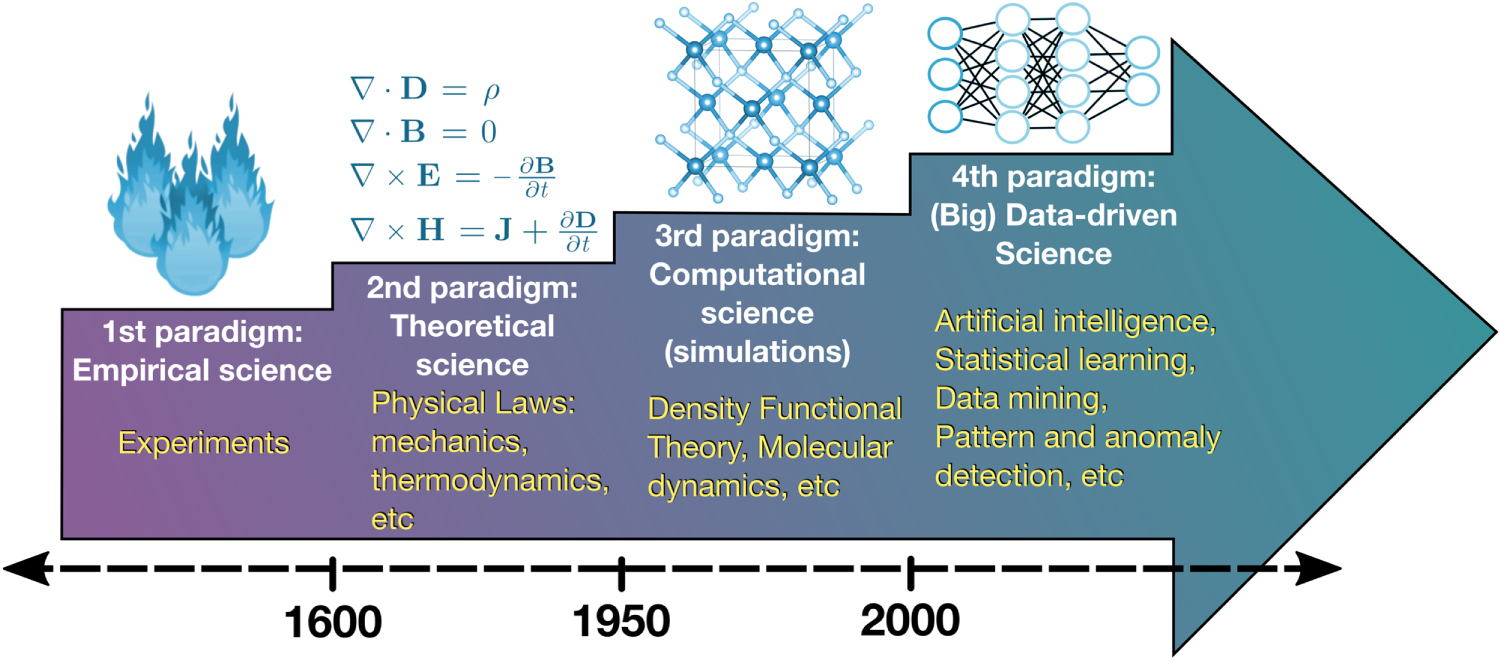
\includegraphics{theory/figures/4th-paradigm-hd.jpg}
  \caption{The four science paradigms: empirical, theoretical, computational, and data-driven. Figure taken from Ref.  \cite{Schleder2019}, which was originally adapted from Ref. \cite{Agrawal2016}.}
  \label{fig:4th-paradigm}
\end{figure}

This chapter aims to provide the necessary understanding of the new research paradigm in the context of computational materials science and novel materials discovery. Starting from the beginning, we will be looking into information gained by \textit{ab initio} calculations, which means "from first-principles". %In particular, it involves a summary of the necessary theory behind the density functional theory, thus leaving most of the quantum-mechanical world untouched.
Since DFT is not a theory one simply understands, we will begin with an initial discussion of why it is difficult to calculate interactions between particles, followed by a review of key approximations and methods regarding the theory. However, even if density functional theory solves some problems, it also introduces new challenges, which will be thoroughly discussed.

Thereafter, we try to provide a logical sequence into the emergence of high-throughput (HT) methods and tools necessary to handle the resulting information. Finally, we review a state-of-the-art approach of novel materials discovery enabled by the new paradigm of big data and data science.

\begin{comment}
\section{The single-electron Schrödringer equation}

We will start of investigating the Schrödinger equation with only one electron \cite{Griffiths2017}
\begin{align}
    i\hslash \frac{\partial \Psi}{\partial t} = -\frac{\hslash^2}{2m}\nabla^2 \Psi + V\Psi
    \label{eq:Schrödinger}
\end{align}
for a convenient external potential $V_{ext}(r)$ that is independent of time. We will try to look for solutions for (\autoref{eq:Schrödinger}) by separating the wavefunction into a space-dependent and time-dependent function
%Most wavefunctions are solutions to (\autoref{eq:Schrödinger}), but if the wavefunction describes a stationary state, the wavefunction has to be an eigenfunction to H for reasons that will become clear shortly.
\begin{align}
  \Psi(r,t) = \psi(r)\phi(t).
  \label{eq:separation}
\end{align}
By inserting ordinary derivatives and dividing each side with equation (\autoref{eq:separation}), our Schrödinger equation (\autoref{eq:Schrödinger}) now reads
\begin{align}
  i\hslash \frac{1}{\phi(t)}\frac{d\phi(t)}{dt} = - \frac{\hslash^2}{2m} \frac{1}{\psi(r)}\nabla^2 \psi + V(r)
\end{align}

Since the potential function $V(r)$ is independent of time, we observe the time and space dependencies of each side and state the fact that both sides has to be constant. Thus, two intriguing equations unveil themselves;
%captivating?
\begin{align}
  i\hslash \frac{1}{\phi(t)}\frac{d\phi(t)}{dt} = E\phi(t)
  \label{eq:time}
\end{align}
and
\begin{align}
  \frac{\hslash^2}{2m} \frac{1}{\psi(r)}\nabla^2 \psi + V(r) = E\psi(r)
  \label{eq:tise}
\end{align}
where the first equation (\autoref{eq:time}) has a general solution $\phi(t) = C \exp (-iEt/\hslash)$ and $C=1$ after normalization, and the second equation (\autoref{eq:tise}) is known as time-independent Schrödinger equation. These two equations are connected through the variable $\varepsilon$.

By utilizing variable separation to get equation (\autoref{eq:separation}), we find that the wavefunction is describing a stationary state with probability density
\begin{align*}
  \lvert \Psi (r,t)\rvert ^2 &= \Psi^*\Psi \\
  &= \Psi^* e^{iEt/\hslash} \Psi e^{-i Et/\hslash} \\
  &= \lvert \Psi (r)\rvert ^2
\end{align*}
that is independent of time. Conveniently, this is also true for every expectation value; they are all constant in time. We can also try to express this in classical terms regarding the Hamiltonian, which in this scenario is defined as
\begin{align}
    \hat{H}(r, p) = \frac{p^2}{2m} + V(r) = -\frac{\hslash^2}{2m}\nabla^2 + V(r)
\end{align}
simplifying equation \autoref{eq:tise} to
\begin{align}
  \hat{H} \psi = E\psi
  \label{eq:tise_nesten}
\end{align}
and we can find the expectation value of the total energy as
\begin{align*}
    \langle H \rangle &= \int \psi^* \hat{H} \psi dr \\
                &= E\int \lvert \Psi \rvert ^2 dr \\
                &= E
\end{align*}
using the fact that expectation values are constant in time for stationary states. Similarly, we can try to estimate the variance of the Hamiltonian,
\begin{align*}
  \sigma_H^2 &= \langle H^2 \rangle - \langle H \rangle ^2 \\
            &= E^2 - E^2 \\
            &= 0
\end{align*}
which appropiately describes that every measurement of the total energy is certain to return the value E.

\subsection{Eigenfunctions}
So far, we have not given an explanation of what a wavefunction is. As a matter of fact, we have actually found an eigenfunction
\begin{align*}
  \psi_\kappa(r,t) = \psi_\kappa e^{-i\varepsilon_\kappa t/\hslash}
\end{align*}
where $\kappa$ denotes the $k$-th eigenfunction and $\varepsilon_\kappa$ is its corresponding energy eigenvalue. The eigenfunctions have distinct energies and have the attribute that they are orthogonal and normalized with respect to
\begin{align*}
  \bra{\psi_\kappa (r,t)} \ket{\psi_{\kappa`} (r,t)} = \delta_{\kappa \kappa'}.
\end{align*}
The state with the lowest energy is called the ground-state, and is where it is most likely to find an electron in a single-electron system with no external potential applied.

A general wavefunction can be generated by a summation of eigenfunctions (such as the eigenfunction in the latter case)
\begin{align}
\Psi(r,t) = \sum_\kappa c_\kappa \psi_{\kappa}(r,t),
\end{align}
where $c_\kappa$ is a constant. A general wavefunction does not necessarily describe stationary states, and consequently does not have distinct energies but is rather represented statistically from the expectation value
\begin{align*}
  E = \sum_{\kappa} \lvert c_\kappa \rvert \varepsilon_\kappa.
\end{align*}
Solving Schrödinger equation for a general wavefunction is rather troublesome. Fortunately, we can use the eigenfunctions instead, transforming equation \autoref{eq:tise_nesten} into time-independent Schrödinger equation for eigenfunctions
\begin{align}
  \hat{H} \psi_{\kappa}(r) = \varepsilon_\kappa \psi_\kappa(r).
\end{align}

The shape of en eigenfunction has normally high spatial symmetri that depends on the symmetri of the potential $V_{ext}(r)$ and the boundary conditions \cite{Persson2020}. The study of how atoms in a crystalline interact with each other is of upmost importance when trying to explain macroscopic consequences.

\end{comment}
\section{Quantum mechanics}
%Before we
%Initially, the method of the calculations can be regarded as a black box where one provides the structure of a material as input, where the black box in return feeds us the outcome in terms of e.g. a different structure. The black box in question is based on a successful theory called density functional theory, which is an approach for predicting physical properties of solid-state systems. %In this and the next section we provide the necessary knowledge to understand what is happening inside the black box, and the quality of the output.

To fully understand what challenges the density functional theory solves, we will need to introduce a few concepts in quantum mechanics. Quantum mechanics is the fundamental theory that describes nature at the microscopic scale. We will only look at the necessary theory needed to understand the DFT, leaving most of the theory in quantum mechanics untouched.

%Leading up to the density functional theory, we will initially introduce a few concepts required to understand it. Specifically, we will need to utilize the theory of quantum mechanics.

%The significance of this will be crystal clear when we later have to interpret information regarding several thousands solid-state systems, and not a single material. In particular, the quality of the output depends on being consistent.



%Before , we will need to investigate how we can calculate the forces acting inside a crystal. Since these forces are happening on a microscopic scale, we will need to utilize the theory of quantum mechanics.

%However, the fundamental theory remains the same and we will start our venture with the Schrödinger equation.


\subsection{The Schrödinger equation}

In principle, we can describe all physical phenomenas of a system with the wavefunction $\Psi(\boldsymbol{r},t)$ and the Hamiltonian $\hat{H}(\boldsymbol{r},t)$, where $\boldsymbol{r}$ is the spatial position and $t$ is the time. Unfortunately, analytical solutions for the the time-dependent Schrödinger equation,
\begin{align}
    i\hslash \frac{\partial}{\partial t} \Psi(\boldsymbol{r},t) = \hat{H}(\boldsymbol{r},t) \Psi(\boldsymbol{r},t),
    \label{eq:tdse}
\end{align}
are extremely rare. More conveniently, we can generate a general wavefunction by a summation of eigenfunctions,
\begin{align}
  \Psi(\boldsymbol{r},t) = \sum_\kappa c_\kappa \psi_\kappa(\boldsymbol{r},t),
\end{align}
where $c_\kappa$ is a constant and $\psi_\kappa$ is the $\kappa$-th eigenfunction. A general wavefunction does not have distinct energies but is rather represented statistically from the expectation value  %necessarily describe stationary states, and consequently does not have distrinct energies but is rather represented statistically from the expectation value
\begin{align}
  \left \langle E \right \rangle = \sum_\kappa \lvert c_\kappa \rvert E_\kappa.
\end{align} Solving the Schrödinger equation for a general wavefunction is rather troublesome. However, for a time independent potential, we can use the eigenfunctions and transform \autoref{eq:tdse} into the time-independent Schrödinger equation for eigenfunctions by separation of variables, resulting in
\begin{align}
  \hat{H}\psi_\kappa(\boldsymbol{r}) = E_\kappa \psi_k(\boldsymbol{r}),
\end{align}
where $E_\kappa$ is the eigenvalue of the $\kappa$-th eigenstate $\psi_\kappa(\boldsymbol{r})$. The eigenfunctions have discrete energies, and the state with the lowest energy is called the ground-state. They have the attribute that they are orthogonal and normalized with respect to
\begin{align}
  \left \langle \psi_\kappa \left(\boldsymbol{r}\right) \rvert \psi_{\kappa`} \left(\boldsymbol{r} \right) \right \rangle = \delta_{\kappa \kappa'}.
\end{align}
For more information, see Ref. \cite{Griffiths2017}.

\subsection{The many-particle Schrödinger equation}
As we extend the theory to include many-particle systems, we will gradually explain and add the different contributions that make up the many-body Hamiltonian. During this process, we will neglect any external potential applied to the system. \begin{comment}Furthermore, we will apply natural units, that is
\begin{itemize}
  \item Reduced planck constant $\hslash  = 1$.
  \item The magnitute of the charge of the electron $e = 1$.
  \item The electron rest mass $m_e = 1$.
  \item The coloumb force constant $(4\pi\varepsilon_0)^{-1}=1$.
\end{itemize}
\end{comment}

If we place a simple electron with mass $m_e$ in a vacuum, it will be in possession of kinetic energy. Instead of just one electron, we can place $N_e$ electrons, and they will together have the total kinetic energy
\begin{align}
  T_e = - \sum_{j=1}^{N_e} \frac{\hslash^2\nabla_j}{2m_e}.
\end{align}
All the electrons are negatively charged, causing repulsive Coulomb interactions between each electron, totalling to
\begin{align}
  U_{ee} = \frac{1}{4\pi\varepsilon_0}\sum_{j=1}^{N_e}\sum_{j'<j} \frac{q^2}{\lvert r_j - r_{j'}\rvert},
  \label{eq:electron-electron}
\end{align}
where $\varepsilon$ is the vacuum permittivity. The summation avoids counting each interaction more than once. Simultaneously, we can place $N_n$ nuclei with mass $m_n$ in the same system, accumulating the kinetic energy
\begin{align}
  T_n = - \sum_{a=1}^{N_n} \frac{\hslash^2\nabla_a}{2m_n}.
\end{align}
As in the example with electrons, the nuclei are also experiencing repulsive interactions between every single nucleus, adding up the total interactions as
\begin{align}
  U_{nn} = \frac{1}{4\pi\varepsilon_0}\sum_{a=1}^{N_n}\sum_{a'<a} \frac{q^2 Z_aZ_{a'}}{\lvert R_a - R_{a'}\rvert }.
\end{align}
where $Z_a$ is the atom number of nuclei number $a$. The system now contains $N_e$ electrons and $N_n$ nuclei, thus we need to include the attractive interactions between the them,
\begin{align}
  U_{en} = - \frac{1}{4\pi\varepsilon_0}\sum_{j=1}^{N_e} \sum_{a=1}^{N_n} \frac{q^2Z_a}{\lvert r_j-R_a\rvert}.
\end{align} Together, these equations comprise the time-independent many-particle Hamiltonian
\begin{align}
  \begin{aligned}
    \hat{H} = &- \sum_{j=1}^{N_e} \frac{\hslash^2\nabla_j}{2m_e}
    - \sum_{a=1}^{N_n} \frac{\hslash^2\nabla_a}{2m_n}
    + \frac{1}{4\pi\varepsilon_0} \sum_{j=1}^{N_e}\sum_{j'<j} \frac{q^2}{\lvert r_j - r_{j'}\rvert} \\
    &+\frac{1}{4\pi\varepsilon_0}\sum_{a=1}^{N_n}\sum_{a'<a} \frac{q^2 Z_aZ_{a'}}{\lvert R_a - R_{a'}\rvert } - \frac{1}{4\pi\varepsilon_0}\sum_{j=1}^{N_e} \sum_{a=1}^{N_n} \frac{q^2Z_a}{\lvert r_j-R_a\rvert}.
  \end{aligned}
\end{align} A few problems arise when trying to solve the many-particle Schrödinger equation. Firstly, the amount of atoms in a crystal is very large. As an example, we can numerically try to calculate \autoref{eq:electron-electron} for a $1$ mm$^3$ silicon-crystal that contains $7\cdot 10^{20}$ electrons. For this particular problem, we will pretend to use the current fastest supercomputer Fugaku \cite{Top500} that can calculate $514$ TFlops (floating operations per second), and we will assume that we need $2000$ Flops to calculate each term inside the sum \cite{Persson2020}, and we need to calculate it $N_e \cdot N_e/2$ times for the (tiny) crystal.
The entire electron-electron interaction calculation would take $2.46 \cdot 10^{19}$ years to finish for a tiny crystal, which is longer than the assumed age of the universe. Thus, the large amount of particles translates into a challenging numerical problem.

%In one cubic-centimeter of a crystal, there are around $10^{23}$ electrons. This number is roughly the same as the number of stars in the universe, grain of sand on all beaches in the world, or currently $1.41\cdot 10^{19}$ times the amount of Home and Away episodes made since 1988.

Secondly, the many-particle Hamiltonian contains operators that have to be applied to single-particle wavefunctions, and we have no prior knowledge of how $\Psi$ depends on the single-particle wavefunctions $\psi_\kappa$.


\subsection{The Born-Oppenheimer approximation}
The many-particle eigenfunction describes the wavefunction of all the electrons and nuclei and we denote it as $\Psi_{\kappa}^{en}$ for electrons (e) and nuclei (n), respectively. The Born-oppenheimer approximation states that nuclei, of substantially larger mass than electrons, can be treated as fixed point charges. According to this assumption, we can separate the eigenfunction into an electronic part and a nuclear part,
\begin{align}
  \Psi_\kappa^{en}(\boldsymbol{r}, \boldsymbol{R}) \approx \Psi_{\kappa}(\boldsymbol{r}, \boldsymbol{R})\Theta_{\kappa}(\boldsymbol{R}),
\end{align}
where the electronic part is dependent on the nuclei. This is in accordance with the assumption above, since electrons can respond instantaneously to a new position of the much slower nucleus, but this is not true for the opposite scenario. By utilizing this approximation, it can be shown that the equation can be separated into an electronic and a nuclear eigenvalue equation,

\begin{align}
      \left( T_e + U_{ee} + U_{en} \right) \Psi_\kappa (\boldsymbol{r},\boldsymbol{R}) &= E_{\kappa}(\boldsymbol{R})\Psi_\kappa(\boldsymbol{r},\boldsymbol{R})\\
      \left(T_n + U_{nn} + E_\kappa (\boldsymbol{R}) \right) \Theta_\kappa(\boldsymbol{R}) &= E_{\kappa}^{en}(\boldsymbol{R})\Theta_\kappa(\boldsymbol{r},\boldsymbol{R}),
\end{align}
where the two equations are coupled by the electronic energy eigenvalue $E_{\kappa}(\boldsymbol{R})$. Since we can consider the nuclei as point charges, it is common to set the kinetic energy of the nuclei, $T_n$, to zero. Thus, the left side of the nuclear eigenvalue equation is shortened down to the terms $\left(U_{nn} + E_\kappa (\boldsymbol{R}) \right)$, which is denoted as the potential energy surface (PES), $E_p(\boldsymbol{R})$.
%From here, one can obtain the electronic and nuclear eigenfunction, with the derivation shown in Appendix \ref{appendix:Born-Oppenheimer}.


\subsection{The Hartree and Hartree-Fock approximations}
\begin{comment}
As we venture along from a one-electron system to a two-electron systen, we encounter a new wavefunction and Hamiltonian that needs to describe two particles, making the two-electron Schrödinger equation read

\begin{align}
  \Big( -\frac{\hslash^2 \nabla_1^2}{2m_e} - \frac{\hslash^2\nabla_2^2}{2m_e}+ \frac{q^2}{\lvert r_1-r_2  \rvert} + V_{ext}(r) \Big) \Psi_\kappa (r_1, r_2) = E_{\kappa} \Psi_\kappa (r_1, r_2),
\end{align}
where the two first terms are the kinetic energies of the electrons, while the third term is a potential that describes the repulsive Coloumb interaction between the two electrons. The last term is the external potential, well known from the earlier scenario with only one electron.
\end{comment}
The next question in line is to find a wavefunction $\Psi(\boldsymbol{r},\boldsymbol{R})$ that describes all of the electrons in the system. The Hartree \cite{Persson2020, DavidSholl2009} approximation to this is to assume that electrons can be described independently, suggesting the \textit{ansatz} for a two-electron wavefunction
\begin{align}
  \Psi_\kappa(\boldsymbol{r}_1,\boldsymbol{r}_2) = A \cdot \psi_1(\boldsymbol{r}_1) \psi_2(\boldsymbol{r}_2),
\end{align}
where $A$ is a normalization constant. This approximation simplifies the many-particle Shrödinger equation a lot, but comes with the downside that the particles are distinguishable and do not obey the Pauli exclusion principle for fermions.

The Hartree-Fock approach, however, overcame this challenge and presented an anti-symmetric wavefunction that made the electrons indistinguishable \cite{Griffiths2017}:
\begin{align}
  \Psi_\kappa(\boldsymbol{r}_1,\boldsymbol{r}_2) = \frac{1}{\sqrt{2}}\Big( \psi_1(\boldsymbol{r}_1) \psi_2(\boldsymbol{r}_2)  - {\psi_1(\boldsymbol{r}_2)\psi_2(\boldsymbol{r}_1)}\Big).
\end{align}
%For systems containing more than one particles, the factor $1/\sqrt{2}$ becomes the Slater determinant and is used to normalize the wavefunction.

\subsection{The variational principle}
So far, we have tried to make the time-independent Schrödinger equation easier with the use of an \textit{ansatz}, but we do not necessarily have an adequate guess for the eigenfunctions and the ansatz can only give a rough estimate in most scenarios. Another approach, namely the \textit{variational principle}, states that the energy of any trial wavefunction is always an upper bound to the exact ground-state energy by definition $E_0$,
\begin{align}
  E_0 = \bra{\psi_0 } H \ket{\psi_0} \leq \bra{\psi}H\ket{\psi} = E
  \label{eq:variational}
\end{align} This enables a minimization of energy in terms of wavefunction parameters. A more thorough walk-through of the variational principle is included in Appendix \ref{appendix:variational-principle}.

\section{The density functional theory}

Hitherto we have tried to solve the Schrödinger equation to get a ground-state wavefunction, and from there we can obtain ground-state properties. One fundamental problem that exists when trying to solve the many-electron Schrödinger equation is that the wavefunction is a complicated function that depends on $3N_e$ variables\footnote{not including spin}.

Hohenberg and Kohn \cite{Hohenberg1964} showed in 1964 that the ground-state density $n_0(r) = \lvert \Psi_0 (r)\rvert$ determines a general external potential, which includes $U_{en}$, up to an additive constant, and thus also the Hamiltonian \cite{Toulouse2019}. From another point of view, the theory states that all physical ground-state properties of the many-electron system are unique functionals of the density \cite{Persson2020}. A consequence of this is that the number of variables is reduced from $3N_e$ to $3$, significantly reducing the computational efforts.

However, the scheme is not without limitations, as the density functional theory (DFT) can only be used to find all the ground-state physical properties if the exact functional of the electron density is known. And $57$ years after Hohenberg and Kohn published their paper, the exact functional still remains unknown.

We will start this section with a brief mention of the Hohenberg-Kohn theorems and their implications, before we delve further into the Kohn-Sham equation.

\subsection{The Hohenberg-Kohn theorems}

\begin{theorem}
  For any system of interacting particles in an external potential $V_{ext}$, the density is uniquely determined.
\end{theorem}

The theorem can be proved by utilizing the variational principle for two different external potentials with the same ground-state density.
The proof is included in Appendix \ref{appendix:theorem1}.

\begin{theorem}
  There exists a variational principle for the energy density functional such that, if $n$ is not the electron density of the ground-state, then $E\left[ n_0 \right] < E\left[ n \right]$.
\end{theorem}

From theorem 1, we know that the external potential is uniquely determined by the density, which in turn uniquely determines the ground-state wavefunction. Therefore, all other observables of the system are uniquely determined and we can express the energy as a function of the density,
\begin{align}
  E[n] = \overbrace{T[n] + U_{ee}[n]}^{F[n]} + U_{en}[n],
  \label{eq:densityfunctional}
\end{align}
where $F[n]$ is an universel functional known as the Hohenberg-Kohn functional. The proof for theorem 2 is found in Appendix \ref{appendix:theorem2}.

\subsection{The Kohn-Sham equation}
So far, we have tried to make the challenging Schrödinger equation less challenging by simplifying it. The last attempt of simplifying it involved the Hohenberg-Kohn's theorems where the theory states that the total ground-state energy can, in principle, be determined exactly once we have found the ground-state density.

In 1965, Kohn and Sham \cite{Kohn1965} reformulated the Hohenberg-Kohn theorems by generating the exact ground-state density $n_0(r)$ using a Hartree-like total wavefunction
\begin{align}
    \Psi(\boldsymbol{r}_1,\boldsymbol{r}_2,..,\boldsymbol{r}_{N_e}) = \psi_1^{KS}(\boldsymbol{r}_2)\psi_2^{KS}(\boldsymbol{r}_2)...\psi_{N_e}^{KS}(\boldsymbol{r}_{N_e}),
\end{align}
where $\psi_j^{KS}(r_j)$ are some auxiliary independent single-particle wavefunctions. However, the Kohn-Sham wavefunctions cannot be the correct single-particle wavefunctions since our ansatz implies an exact density
\begin{align}
  n(\boldsymbol{r}) = \sum_{j=1}^{N_e}\lvert \psi_j^{KS}(\boldsymbol{r})\rvert^2.
\end{align}
Recalling that equation \autoref{eq:densityfunctional} describes the total energy as a functional of the density,
\begin{align}
  E[n] = T[n] + U_{ee}[n] + U_{en}[n],
\end{align}
we try to modify it to include the kinetic energy $T_s[n]$ and the interaction energy $U_s[n]$ of the auxiliary wavefunction, with the denotation $s$ for single-particle wavefunctions.
\begin{align*}
  E[n] &= T[n] + U_{ee}[n] + U_{en}[n] + \left( T_s[n] - T_s[n] \right) + \left( U_s[n] - U_s[n] \right) \\
  &= T_s[n] + U_{s}[n] + U_{en}[n] + \underbrace{\left(T[n] - T_s[n] \right) + \left( U_{ee}[n] - U_s[n] \right)}_{E_{xc}[n]}.
\end{align*}
Here we have our first encounter with the \textit{exchange-correlation energy}
\begin{align}
  E_{xc}[n] = \Delta T + \Delta U = \left(T[n] - T_s[n] \right) + \left( U_{ee}[n] - U_s[n] \right),
\end{align}
which contains the complex many-electron interaction. For non-interacting systems, $E_{xc}[n]$ is conveniently zero, but in interacting systems it most likely is a complex expression. However, one can consider it as our mission to find good approximations to this term, as the better approximations, the closer we get to the exact expression.

The exact total energy functional can now be expressed as
\begin{align}
  \begin{aligned}
  E[n]
  &= \overbrace{\sum_j \int \psi_j^{KS*} \frac{-\hslash^2\nabla^2}{2m} \psi_j^{KS}d\boldsymbol{r}}^{T_s[n]} + \overbrace{\frac{1}{2}\frac{1}{4\pi\varepsilon_0}\int \int q^2\frac{n(\boldsymbol{r})n(\boldsymbol{r}')}{\lvert \boldsymbol{r}-\boldsymbol{r}'\rvert} d\boldsymbol{r}d\boldsymbol{r}'}^{U_s[n]}
  \\ &+ \underbrace{\int V_{en}(\boldsymbol{r})n(\boldsymbol{r})d\boldsymbol{r}}_{U_{en}[n]} + \underbrace{\left(T[n] - T_s[n] \right) + \left( U_{ee}[n] - U_s[n] \right)}_{E_{xc[n]}},
  \end{aligned}
\end{align}
given that the exchange-correlation functional is described correctly. By utilizing the variational principle, we can now formulate a set of Kohn-Sham single-electron equations,
\begin{align}
  \left\{ -\frac{\hslash^2}{2m_e}\nabla^2_s + V_H(\boldsymbol{r}) + V_{en}(\boldsymbol{r}) + V_{xc}(\boldsymbol{r}) \right\} \psi_s^{KS}(\boldsymbol{r}) = \epsilon_s^{KS} \psi_s^{KS}(\boldsymbol{r}),
  \label{eq:singleKS}
\end{align}
where $V_{xc}(\boldsymbol{r})=\partial E_{xc}[n]/\partial n(\boldsymbol{r})$ and $V_{H}(\boldsymbol{r})=\frac{1}{4\pi\varepsilon_0}\int q^2 \frac{n(\boldsymbol{r'})}{\lvert \boldsymbol{r} - \boldsymbol{r}'\rvert} d\boldsymbol{r}'$ is the Hartree potential describing the electron-electron interaction.
It is worth noticing that $V_H(\boldsymbol{r})$ allows an electron to interact with itself, resulting in a self-interaction contribution, however, this can be taken care of in $V_{xc}$.

Finally, we can define the total energy of the system according to Kohn-Sham theory as
\begin{align}
  E[n] = \sum_{j}\epsilon_j^{KS}-\frac{1}{2}\frac{1}{4\pi\varepsilon_0}\int \int q^2 \frac{n(\boldsymbol{r})n(\boldsymbol{r}')}{\lvert \boldsymbol{r} - \boldsymbol{r}' \rvert} d\boldsymbol{r}d\boldsymbol{r}' + E_{xc}[n] - \int V_{xc}(\boldsymbol{r})n(\boldsymbol{r})d\boldsymbol{r}.
\end{align}
If $V_{xc}$ is exact, and $E[n]$ gives the true total energy, we still do not know if the energy eigenvalues $\epsilon_s^{KS}$ are the true single-electron eigenvalues. However, there exists one exception, which is that the highest occupied eigenvalue of a finite system has to be exact if the density is exact.

The only task that is left for us now is to find the exact expression for $E_{xc}[n]$ as a functional of the density $n(r)$. With that expression, we would be able to calculate the total energies of any material. %, and most likely solve a few of the biggest puzzles in the history of humankind.
Unfortunately, the exchange-correlation potential is unknown for most systems.

It is possible to solve the Kohn-Sham equations by applying a self-consistent field method. This is a computational scheme, and for further details, one can consult the Appendix \ref{appendix:self-consistent}.

%In this approximation we have used Hartree energy where the self-interaction correction is neglected, raising less accurate results. It is possible to use other approximations for $T_s[n]$ and $U_s[n]$ than Hartree wavefunctions, and good approximations will result in a low $E_{xc}[n]$ because $T_s[n]$ and $U_s[n]$ will get closer and closer to the true values.


%The next step in finding the KS-equation is to utilize the variational principle in the purpose of finding the ground-state energy. First one minimises the total energy with respect to each of the wavefunctions with the constraint that the wavefunctions should be orthonormalized;
%\begin{align*}
%  \frac{\partial }{\partial \psi_j^{*} (\boldsymbol{r})}E[n] &= \sum_{i,j}\lambda_{ij}\int \psi_i^{s*}(\boldsymbol{r}_i)\psi_j^{s}(\boldsymbol{r}_j)d\boldsymbol{r}d\boldsymbol{r}_j\\
%  \frac{\partial }{\partial \psi_j^{*} (\boldsymbol{r})}E[n] &= \lambda_j\psi_j^s (\boldsymbol{r}_j)
%\end{align*}

\subsection{The exchange-correlation energy}


There is one scenario for which we can derive the exact expression of the exchange-correlation functional, namely the \textit{homogeneous electron gas} (HEG). However, this has a natural cause, since by definition $n(\boldsymbol{r})$ is constant for this situation. Given that it is the variations of electron density that are the foundation of material properties, the usefulness of HEG is limited. The \textit{local density approximation} (LDA) is an approximation based on this approach, where the local density is the only variable used to define the exchange-correlation functional. Specifically, we can set the exchange-correlation potential at each position to be the known exchange-correlation potential from homogeneous electron gas at the electron density observed at that position \cite{Kohn1965}:
\begin{align}
  V_{xc}(\boldsymbol{r}) = V_{xc}^{\text{electron gas }}\left[n(\boldsymbol{r})\right].
\end{align}
This is the simplest and most known approximation to the exchange-correlation functional, and accordingly, it has a few drawbacks. One of them is the incomplete cancellation of the self-interaction term, which leads to a repulsion that may cause artificial repulsion between electrons, and hence increased electron delocalization \cite{Allen2014}. In addition, LDA has proven challenging to use when studying atoms and molecules because of their rapidly varying electron densities, however, the LDA is seen as successful for bulk materials because of the slowly varying electron density \cite{DavidSholl2009}. Considering the relatively low computational cost and relatively high accuracy, the LDA overall makes a good model for estimation of the exchange-correlation functional for bulk materials.

In the light of the merits of the LDA, an extensive search for new approximations was launched. The \textit{generalized gradient approximation} (GGA) is an extension of the LDA, which includes the gradient of the density
\begin{align}
  V_{xc}^{GGA}(\boldsymbol{r}) = V_{xc}\left[ n(\boldsymbol{r}), \nabla n (\boldsymbol{r})\right].
\end{align}
The GGA is a good approximation for the cases where the electron density varies slowly, but faces difficulties in many materials with rapidly varying gradients in the density, causing the GGA to fail. Thus, the annotation \textit{generalized} in GGA is set to include the different approaches to deal with this challenge. Two of the most commonly implemented GGA functionals are the non-empirical approaches Perdew-Wang 91 (PW91) \cite{Perdew1992} and Perdew-Burke-Ernzerhof (PBE) \cite{Perdew1996}.

Both LDA and GGA are commonly known to severely underestimate the band gaps of semiconductor materials, in addition to incorrectly predicting charge localizations originating from narrow bands or associated with local lattice distortions around defects \cite{Freysoldt2014}. The latter limitation is thought to be due to self-interaction in the Hartree potential in \autoref{eq:singleKS}.
\begin{comment}
To improve the accuracy of excited state properties estimations, other methods have been developed. Tran and Blaha (TB) \cite{Tran2009} adapted the exchange potential suggested by Becke-Roussel (BR) \cite{Becke2006} that leads to band gaps close to experimental values while still using a cheap semilocal method \cite{Koller2011}. The modified TB-mBJ version introduces a parameter relative to the BJ version,
\begin{align}
    V_{xc}^{TB-mBJ}(\boldsymbol{r}) =  c\cdot V_{xc}^{BR}(\boldsymbol{r}) + (3c-2) \frac{1}{\pi} \sqrt{\frac{5}{6}} \sqrt{\frac{t(\boldsymbol{r})}{\rho(\boldsymbol{r})}},
\end{align}
where $\rho$ is the electron density, $t$ is the kinetic-energy density, $V_{xc}^{BR}$ is the Becke-Roussel exchange potential and $c$ is the parameter that changes weights of the BJ potential and is fit to experimental data.
\end{comment}
Hybrid functionals intermix exact Hartree-Fock exchange with exchange and correlation from functionals based on the LDA or GGA.
Hartree-Fock theory ignores correlation effects, but accounts for self-interaction and treats exchange as exact.
Since LDA/GGA and Hartree-Fock supplement each other, they can be used as a combination for hybrid-functionals resulting in some cancellation of the self-interaction error. Becke \cite{Becke1993} introduced a $50\%$ Hartree-Fock exact exchange and
$50\%$ LDA energy functional, while Perdew \textit{et al.} \cite{Perdew1996a} altered it to $25\%-75\%$ and favoring PBE-GGA instead of LDA.

The inclusion of Hartree-Fock exchange improves the description of localized states but requires significantly more computational power for large systems. Another method called the \textit{GW} approximation includes a screening of the exchange interaction \cite{Aryasetiawan1998}, but has a computational price that does not necessarily defend its use. Thus, the real challenge is to reduce the computational effort while still producing satisfactory results. Heyd \textit{et al.} \cite{Heyd2003} suggested separating the non-local Hartree-Fock exchange into a short- and long-range portion, incorporating the exact exchange in the short-range contribution. The separation is controlled by an adjustable parameter $\omega$, which was empirically optimized for molecules to $\omega = 0.15$ and solids to $\omega = 0.11$ and are known as the HSE03 and HSE06 (Heyd-Scuseria-Ernzerhof), respectively \cite{Krukau2006}. The functionals are expressed as
\begin{align}
  E_{xc}^{HSE} = aE_{x}^{\text{HF,SR}}(\omega) + (1-a)E_x^{\text{PBE,SR}}(\omega) + E_x^{\text{PBE,LR}}(\omega) + E_c^{\text{PBE}},
\end{align}
where $a=1/4$ is the Hartree-Fock mixing constant and the abbreviations SR and LR stands for short range and long range, respectively.

Hence, hybrid-functionals are \textit{semi-empirical} functionals that rely on experimental data for accurate results. They give accurate results for several properties, such as energetics, bandgaps and lattice parameters, and can fine-tune parameters fitted to experimental data for even higher accuracy.

Furthermore, the computational effort required for the hybrid-functionals is significantly larger than for non-empirical functionals such as LDA or GGA. Krukau \textit{et al.} \cite{Krukau2006} reported a substantial increase in computational cost when reducing the parameter $\omega$ from $0.20$ to $0.11$ for 25 solids, and going lower than $0.11$ demanded too much to actually defend its use.
\begin{comment}
Unfortunately, an area where both GGA and hybrid functionals are reportedly inadequate is in calculating the dispersion interactions \cite{Klimes2009}. Many implementations have been developed to deal with this vulnerability, with one of them being the non-local van der Waals density functional (vdW-DF) \cite{Dion2004}
\begin{align}
  E_{xc} = E_{x}^{GGA} + E_{c}^{\text{LDA}} + E_{c}^{nl},
\end{align}
where $E_{x}^{GGA}$ is GGA exchange energy \cite{Klimes2009}.
\end{comment}
\subsection{Limitations of the DFT}

If we had known the exact exchange-correlation functional, the density functional theory would yield the exact total energy. Alas, that is not the case and we are bound to use approximations in the forms of functionals. What is common for all approximations is that they are specifically designed to solve one given optimization in DFT, therefore it is not necessarily one functional that is considered superior in all fields of interest. One could consider that the hybrid functionals due to a high accuracy overall should be dominant, but that is only if one has the computational capacity required. The accuracy of calculations depends on which functional is used, and normally a higher accuracy means the use of a more complex and computationally demanding functional.

Additionally, one can almost never be certain if a DFT-calculation has found a local or global minimum. There is an unknown associated uncertainty of every calculation, which has to be taken into consideration. Nonetheless, density functional theory is considered a very successful approach and Walter Kohn was awarded the Nobel Price in chemistry in 1998 for his development of the density-functional theory \cite{Freitas1999}. It has matured into the undisputed choice of method for electronic structure calculations \cite{Schleder2019}. It is especially regarded as successful in contexts where DFT can make important contributions to scientific questions where it would be essentially impossible to determine through experiments \cite{DavidSholl2009}. %One can only hope that the future will be as bright as the past, and that this successful theory provides incentives for further growth in the next generation.

\section{High-throughput information storage}


Fuelled by the widespread application of DFT in material science, we observe an increase in computational capacity due to advances in simulation methods, computational science and technologies \cite{Schleder2019}. The time required for calculations has been reduced substantially and enables more time to be spent on simulation setup and analysis. Ultimately, this has led to a new type of workflow called high-throughput (HT) \cite{Yang2017}, where one can automate input creation and perform several (up to millions) simulations in parallel instead of performing many manually-prepared simulations. The HT engines are required to be fast and accurate, otherwise, the purpose of their existence is lost. We will in this thesis mainly focus on high throughput in the context of first-principles DFT calculations.

Normally, the implementation of HT-DFT methods is done in three steps. In the first step, we perform thermodynamic or electronic structure calculations for a large number of materials. For the second step, we store the information gathered in a systematic database, normally known as a material repository. For the third and final step, we characterize and select novel materials or analyze and extract new physical insight \cite{Schleder2019}. In general, the two first steps are performed on high-performance computers (HPC), and are defining for the third step due to the vast amount of interesting properties of materials. Importantly, one needs to consider the ultimate goal in step three initially before deciding upon materials and properties to calculate.

One of the largest government-funded projects is the $2011$ launched Material Genome Initiative (MGI) \cite{Warren2018} which seeks to accelerate the discovery, design, development and deployment of novel materials through the creation of a materials innovation infrastructure.
As a result, we have seen an intensive implementation of material repositories that facilitate sharing and distribution of step $1$ and $2$, with the ultimate goal of storing calculated properties of all feasible structures of materials \cite{Schuett2020}.
Examples include AFLOW \cite{Curtarolo2012, Curtarolo2012a, Calderon2015}, Materials Project \cite{Jain2013, Jain2018} , OQMD \cite{Saal2013, Kirklin2015} and JARVIS-DFT \cite{Choudhary2020}.
On the other hand, we find a less diverse selection of experimental databases, with perhaps the most known being the Inorganic Crystal Structure Database (ICSD) \cite{Allen1987}.

In this section, we describe a few of the most widely known high-throughput databases, codes and tools, with an emphasis on what the particular specialty of each database is.

\subsection{Materials project}

Materials project \cite{Jain2013, Jain2018} is an open-source project that is based on the Vienna Ab Initio Software Package (VASP) \cite{Kresse1996}, and offers a variety of properties of over one hundred thousand inorganic crystalline materials. It is known as the initiator of materials genomics and has as its mission to accelerate the discovery of new technological materials, with an emphasis on batteries and electrodes, through advanced scientific computing and innovative design.

 %Some features, eg. density of state (dos), bandstructure, Pourbaix diagram etc., are characterized by using the module pymatgen.

Every compound has an initial relaxation of cell and lattice parameters performed using a $1000$ / (number of atoms in the cell) k-point mesh to ensure that all properties calculated are representative of the idealized unit cell for each respective crystal structure \cite{Ferrenti2020}. The functional GGA is used to calculate band structures, while for transition metals, a $+U$ correction is applied to correct for correlation effects in d- and f-orbital systems that are not addressed by GGA calculations \cite{Wang2006}.

To address that many compounds are not thermodynamically stable, which means that they do not appear on any phase stability diagrams \cite{Sun2016}, an additional metric has been added. This metric is based on a convex hull analysis, where compounds on the convex hull are stable, while compounds above the hull in terms of energy are metastable \cite{Jain2018}. This is denoted as energy above hull (E Above Hull), where a value of zero is defined as the most stable phase at a given composition, while larger positive values indicate increased instability.

%The thermodynamic stability for each phase with respect to decomposition, is also calculated.
Each material contains multiple computations for different purposes, resulting in different 'tasks'. The reason behind this is that each computation has a purpose, such as to calculate the band structure or energy. Therefore, it is possible to receive several tasks for one material.

\subsection{AFLOW}

The AFLOW\cite{Curtarolo2012, Curtarolo2012a, Calderon2015} repository is an automatic software framework for the calculations of a wide range of inorganic material properties. They utilize the GGA-PBE functional within VASP with projector-augmented wavefunction (PAW) potentials to relax twice and optimize the ICSD-sourced structure. They are using a $3000$ to $6000$ / (number of atoms in the cell) $k$-point mesh, indicating a more computationally expensive calculation compared to the Materials Project \cite{Ferrenti2020}.
Next, the band structure is calculated with an even higher $k$-point density, in addition to the $+U$ correction term for most occupied d- and f-orbital systems \cite{Setyawan2010}. Furthermore, they apply a standard fit gathered from a study of DFT-computed versus experimentally measured band gap widths to the initial calculated value, obtaining a fitted band gap \cite{Setyawan2011}.

\subsection{Open Quantum Materials Database}

The Open Quantum Materials Database (OQDM) \cite{Saal2013, Kirklin2015} is a free and available database of DFT-calculations. It contains thermodynamic and structural properties of more than $600.000$ materials, including all unique compounds in the Inorganic Crystal Structure Database (ICSD) that consists of less than $34$ atoms \cite{Ferrenti2020}.

The DFT calculations are performed with the VASP software whereas the electron exchange and correlation are described with the GGA-PBE, while using the PAW potentials. They relax a structure using $4000-8000$ / (number of atoms in the cell) $k$-point mesh, indicating an even more computationally expensive calculation than AFLOW \cite{Ferrenti2020}. Several element-specific settings are included such as using the $+U$ extension for various transition metals, lanthanides and actinides. In addition, any calculation containing 3d or actinide elements is spin-polarized with a ferromagnetic alignment of spins to capture possible magnetism. However, the authors note that this approach does not capture complex magnetic properties such as antiferromagnetism, which has been found to result in substantial errors for the formation energy \cite{Stevanovic2012}.

\subsection{JARVIS}

Joint Automated Repository for Various Integrated Simulations (JARVIS) - DFT \cite{Choudhary2020} is an open database based on the VASP \cite{Kresse1996} software to perform a variety of material property calculations. It consists of roughly $40.000$ 3D and $1.000$ 2D materials using the vdW-DF-OptB88 van der Waals (vdW) functional, which was originally designed to improve the approximation of properties of two-dimensional van der Waals materials, but was also shown to be effective for bulk materials \cite{Thonhauser2007, Klimes2011}. The functional has yielded accurate predictions for lattice-parameters and energetics for both vdW and non-vdW bonded materials  \cite{Choudhary2018}.

Structures included in the data set are originally taken from the Materials Project, and then re-optimized using the OPT-functional. Finally, the combination of the OPT and modified Becke-Johnson (mBJ) functionals are used to obtain a representative band gap of each structure \cite{Choudhary2018a}. %, since both have shown unprecedented accuracy in the calculation of band gap compared to any other DFT-based calculation methods \cite{Choudhary2018a}.
The JARVIS-DFT database is part of a bigger platform that includes JARVIS-FF, which is the evaluation of classical forcefield with respect to DFT-data, and JARVIS-ML, which is a repository of machine learning model parameters and descriptors.
%which consists of 25 machine learning descriptors to predict properties of materials.
In addition, JARVIS-DFT also includes a data set of 1D-nanowire and 0D-molecular materials, which is not yet publically distributed.

\section{Materials informatics}

Despite a computationally demanding step $1$ and a sophisticated database architecture defined in step $2$, the third step remains more important in the discovery of novel materials. In the third step, we apply constraints to the database in order to filter or select the best candidates according to the desired attributes \cite{Schleder2019}, and is referred to as data \textit{mining} and data \textit{screening}. To achieve the most insight, we normally apply the constraints in a sequential manner to identify any potential underlying trend. The materials that satisfy the first constraint move on to the next round, while the rest are eliminated from further consideration. The constraints can be applied either by the understanding of properties, human intuition, or through close interaction with a machine learning (ML) algorithm, where the latter will be extensively studied in the next chapter.

\begin{figure}[ht!]
  \centering
  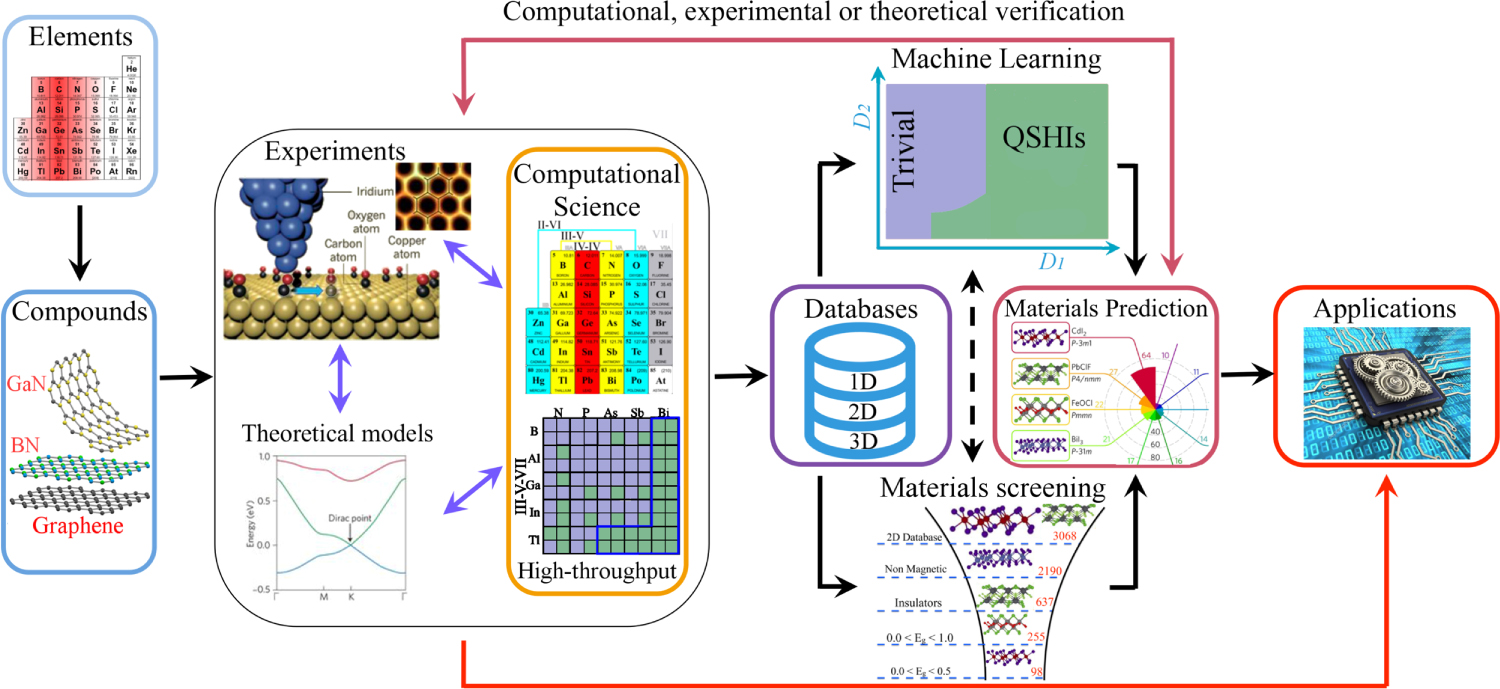
\includegraphics{theory/figures/ht-workflow.jpg}
  \caption{Schematic representation of the workflow of novel materials discovery.  Figure taken from Ref. \cite{Schleder2019}, which was originally adapted from Refs. \cite{Mounet2018, Acosta2018, Polini2013}.}
  \label{fig:ht-workflow}
\end{figure}

Together, the three steps resemble \autoref{fig:ht-workflow}. From building compounds based on elements, calculating theoretical, computational, and experimental properties, storing the information in databases, and applying material screening and machine learning, to finally receiving a material prediction. If the material prediction is verified iteratively by many independent sources, the time to market for new technologies based on a new material takes approximately $20$ years \cite{Eagar1995, Schleder2019}.

\noindent Importantly, the data-driven paradigm enables a new approach for novel material discovery. The traditional approach, namely the \textit{direct approach}, relies on the calculation of properties given the structure and composition of a material, such that the search for eligible candidates exhibiting the target property is performed tediously case by case. In other words, find the answer to what is the property of a given material. However, the \textit{inverse approach} is of integral importance in this work: given the desired property, what material can present it \cite{Schleder2019}?

The application of machine learning and data-driven techniques to material science has developed into a new field named \textit{materials informatics} \cite{Rajan2005}. Alex Szalay, director of the US National Virtual Observatory project, described informatics for astronomy in $2003$ as the following:
\begin{quote}
   ``Science was originally empirical, like Leonardo making wonderful drawings of nature. Next came the theorists who tried to write down equations that explained observed behaviors, like Kepler or Einstein. Then, when we got to complex enough systems like the clustering of a million galaxies, there came the computer simulations – the computational branch of science. Now, we are getting into the data exploration part of science, which is kind of a little bit of them all'' Alex Szalay \cite{Szalay2003}
\end{quote}
\noindent The formulation is true also for materials informatics, where the scope is to discover relations between known standard features and material properties through a combination of \emph{a bit of everything}.

\subsection{Materials informatics software packages}

In practice, several software packages exist for the purpose of generating, describing, visualizing, calculating, or predicting properties of materials.

The Atomic Simulation Environment (ASE) is an environment in the Python programming language that includes several tools and modules for setting up, modifying and evaluate atomistic simulations \cite{Larsen2017}. It is in particular used together with the Computational Materials Repository (CMR) \cite{Landis2012}.

Another commonly used module is the Python Materials Genomics (pymatgen) \cite{Ong2013}. This is a well-documented open module with both introductory and advanced use case examples written in Jupyter Notebook for easy reproducibility, and is integrated with the Materials Project. %RESTful API.

An increasingly popular library is Matminer \cite{Ward2018}, which is an open-source toolkit for material analysis written in Python. Matminer is powered by a group known as \textit{Hacking Materials Research Group}\footnote{Project's Github site: https://github.com/hackingmaterials.}. Matminer provides modules to extract data information from a wide variety of databases. Additionally, they provide the tools to construct possibly thousands of features from calculations based on a materials composition, structure and DFT-calculations, and have modules for visualization and automatic machine learning.

AFLOW-ML \cite{Isayev2017} is an API that uses machine learning to predict thermomechanical and electronic properties based on the chemical composition and atomic structure alone, which they denote as \textit{fragment descriptors}. They start with applying a classification model to predict if a compound is either a metal or an insulator, where the latter is confirmed with an additional regression model to predict the band gap width. To be able to predict properties on an independent data set, they utilize a fivefold cross-validation process for each model. They report a $93$\% prediction success rate of their initial binary classification model, whereas the majority of the wrongful predictions are narrow-gap semiconductors. It has been found that $93$\% of the machine-learning-derived values are within $25$\% of the DFT $+U$-calculated band gap width \cite{Ferrenti2020}.

%The authors does not compare their predicted band gap to experimental values, but it is found that $93$\% of the machine-learning-derived values are within $25$\% of the DFT $+U$-calculated band gap width \cite{Ferrenti2020}.

\subsection{Associated challenges with materials informatics}

%Despite the new and promising methods recently

Despite the promising methods recently developed for novel materials discovery, there are considerable challenges that need to be addressed.

The data generated by HT-DFT are estimates of varying degrees depending on functional applied. In the perspective of this work, we emphasize the underestimation of predicted band gaps. In particular, we find that the (arguably) most popular materials science database Materials Project estimate band gaps with the GGA functional (+U for transition metals). If we were to use their data, it is important to validate its quality, such that we can draw conclusions with the correct information at hand.

Furthermore, out of the (so far) $118$ discovered elements, there are potentially millions of combinations that constitute distinct materials. Only a small fraction of these materials have their basic properties determined \cite{Springer2017}. If we were to involve all combinations of surfaces, nanostructures and inorganic materials, the complexity would increase substantially. This has two consequences. Firstly, due to the small number of determined properties, we are bound to continue with estimates for probably a long time. Perhaps more optimistic is the second consequence, since it is reasonable to believe that materials with promising properties are still to be discovered in almost every field \cite{Pedregosa2012}.

We are at the beginning of a new era, with new technological advances happening every day. By acknowledging and overcoming the challenges, we believe the future is looking bright for material informatics.
